\documentclass[11pt,a4paper]{scrartcl}
% =====================================================================
%  pds-apuntes.tex — Estilo común de apuntes y hojas de ejercicios.
%
%  Uso (desde teoría/Tx/apuntes/ o teoría/Tx/ejercicios/):
%     \documentclass[11pt,a4paper]{scrartcl}   % o scrreprt
%     % =====================================================================
%  pds-apuntes.tex — Estilo común de apuntes y hojas de ejercicios.
%
%  Uso (desde teoría/Tx/apuntes/ o teoría/Tx/ejercicios/):
%     \documentclass[11pt,a4paper]{scrartcl}   % o scrreprt
%     % =====================================================================
%  pds-apuntes.tex — Estilo común de apuntes y hojas de ejercicios.
%
%  Uso (desde teoría/Tx/apuntes/ o teoría/Tx/ejercicios/):
%     \documentclass[11pt,a4paper]{scrartcl}   % o scrreprt
%     \input{../../comun/pds-apuntes}
%     \tema{1}{Introducción: señales y sistemas}
%     \begin{document} \cabecera{Apuntes} ... \end{document}
%  Compilar con:  latexmk -xelatex  (o «make» desde teoría/)
% =====================================================================

\input{../../comun/pds-comun.tex}

\usepackage[a4paper, top=2.6cm, bottom=2.6cm, left=2.5cm, right=2.5cm,
            headheight=1.1cm]{geometry}
\usepackage{fontspec}
\usepackage{unicode-math}
\setmainfont{LibertinusSerif}[Extension=.otf, UprightFont=*-Regular, BoldFont=*-Semibold,
  ItalicFont=*-Italic, BoldItalicFont=*-SemiboldItalic]
\setsansfont{FiraSans}[Extension=.otf, UprightFont=*-Regular, BoldFont=*-SemiBold,
  ItalicFont=*-Italic, BoldItalicFont=*-SemiBoldItalic, Scale=MatchLowercase]
\setmonofont{FiraMono}[Extension=.otf, UprightFont=*-Regular, BoldFont=*-Medium, AutoFakeSlant=0.15, Scale=0.85]
\setmathfont{LibertinusMath-Regular.otf}

\usepackage{microtype}
\usepackage{enumitem}
\usepackage{multicol}
\setlist{itemsep=2pt, topsep=4pt}
\usepackage{caption}
\captionsetup{font=small, labelfont={sf,bf,color=pdsazul}, labelsep=period}
\usepackage{subcaption}
\usepackage[most]{tcolorbox}
\usepackage{environ}
\usepackage{scrlayer-scrpage}
\usepackage[hidelinks, unicode]{hyperref}
\usepackage[spanish, noabbrev]{cleveref}

% Títulos en Fira Sans con el azul de la asignatura
\setkomafont{disposition}{\sffamily\bfseries\color{pdsazul}}
\setkomafont{descriptionlabel}{\sffamily\bfseries}
\setlength{\parindent}{0pt}
\setlength{\parskip}{0.55\baselineskip plus 2pt}
\linespread{1.05}

% ---------------------------------------------------------------------
%  Datos del tema y cabeceras
% ---------------------------------------------------------------------
\newcommand{\numtema}{}
\newcommand{\nombretema}{}
\newcommand{\tema}[2]{\renewcommand{\numtema}{#1}\renewcommand{\nombretema}{#2}}

\pagestyle{scrheadings}
\clearpairofpagestyles
\ihead{\sffamily\small\color{pdsgris}\asignatura}
\ohead{\sffamily\small\color{pdsgris}Tema~\numtema. \nombretema}
\ifoot{\sffamily\small\color{pdsgris}\grado}
\ofoot{\sffamily\small\pagemark}
\setkomafont{pagehead}{\normalfont}
\setkomafont{pagefoot}{\normalfont}

% \cabecera{Apuntes|Ejercicios|...} : bloque de título de la primera página
\newcommand{\cabecera}[1]{%
  \thispagestyle{plain.scrheadings}%
  \noindent
  \begin{minipage}[c]{2.2cm}
    
\includegraphics[width=1.9cm]{../../comun/ucm.png}
  \end{minipage}%
  \begin{minipage}[c]{\dimexpr\linewidth-2.2cm}
    \sffamily
    {\small\color{pdsgris}\grado\par \asignatura\ · \curso\par}
    \vspace{4pt}
    {\Large\bfseries\color{pdsazul}#1\par}
    {\large\bfseries Tema~\numtema. \nombretema\par}
    \vspace{2pt}
    {\small\color{pdsgris}\autores\par}
  \end{minipage}\par
  \vspace{6pt}{\color{pdsazul}\rule{\linewidth}{0.8pt}}\par\vspace{4pt}}

% ---------------------------------------------------------------------
%  Cajas: definición, propiedad, ejemplo, nota, «en código»
% ---------------------------------------------------------------------
\tcbset{pdsbase/.style={enhanced, breakable, boxrule=0pt, arc=1.5pt, left=8pt, right=8pt,
    top=5pt, bottom=5pt, fonttitle=\sffamily\bfseries\small, coltitle=white,
    before skip=8pt, after skip=8pt}}
\newtcbtheorem[number within=section]{definicion}{Definición}%
  {pdsbase, colback=pdsfondo, colframe=pdsazul, borderline west={2.5pt}{0pt}{pdsazul}}{def}
\newtcbtheorem[use counter from=definicion]{propiedad}{Propiedad}%
  {pdsbase, colback=pdsfondo, colframe=pdsazul!75, borderline west={2.5pt}{0pt}{pdsazul!75}}{prop}
\newtcbtheorem[use counter from=definicion]{ejemplo}{Ejemplo}%
  {pdsbase, colback=pdsverde!5, colframe=pdsverde, borderline west={2.5pt}{0pt}{pdsverde}}{ej}
\newtcolorbox{nota}[1][Nota]{pdsbase, colback=pdsnaranja!7, colframe=pdsnaranja,
  title={#1}, borderline west={2.5pt}{0pt}{pdsnaranja}}
\newtcolorbox{importante}[1][Importante]{pdsbase, colback=pdsrojo!5, colframe=pdsrojo,
  title={#1}, borderline west={2.5pt}{0pt}{pdsrojo}}
\newtcolorbox{encodigo}[1][En código]{pdsbase, colback=white, colframe=pdsgris,
  title={#1}, borderline west={2.5pt}{0pt}{pdsgris}}

\lstset{basicstyle=\ttfamily\small}
\renewcommand{\codigoetiqueta}[1]{{\sffamily\small\bfseries\color{pdsgris}#1}}

% ---------------------------------------------------------------------
%  Hojas de ejercicios: \begin{ejercicio} ... \end{ejercicio} y
%  \begin{solucion} ... \end{solucion} (solo se imprime si se define
%  \SOLUCIONES antes de cargar el documento; ver *-Soluciones.tex)
% ---------------------------------------------------------------------
\newif\ifsoluciones
\ifdefined\SOLUCIONES \solucionestrue \fi
\newcounter{ejercicio}
\newenvironment{ejercicio}[1][]{%
  \refstepcounter{ejercicio}\par\vspace{6pt}%
  \noindent{\sffamily\bfseries\color{pdsazul}Ejercicio~\theejercicio}%
  \if\relax\detokenize{#1}\relax\else\ {\sffamily\color{pdsgris}(#1)}\fi\quad}%
  {\par}
\NewEnviron{solucion}{%
  \ifsoluciones
    \begin{tcolorbox}[pdsbase, colback=pdsverde!4, colframe=pdsverde,
      borderline west={2.5pt}{0pt}{pdsverde}, title={Solución}]
      \BODY
    \end{tcolorbox}
  \fi}
% \begin{incisos}[columnas] ... \end{incisos}: apartados a), b)... de un
% enunciado repartidos en columnas (3 por defecto)
% (con una sola columna no se usa multicols, que necesita al menos dos)
\newenvironment{incisos}[1][3]{\par\vspace{-2pt}%
  \ifnum#1>1 \def\finincisos{\end{multicols}}\begin{multicols}{#1}\raggedcolumns\raggedright
  \else\def\finincisos{}\fi
  \begin{enumerate}[label=\alph*), itemsep=3pt, topsep=0pt]}%
  {\end{enumerate}\finincisos\vspace{-4pt}}
\newcommand{\herramienta}[1]{\emph{Herramienta interactiva:} \texttt{herramientas/#1}}

%     \tema{1}{Introducción: señales y sistemas}
%     \begin{document} \cabecera{Apuntes} ... \end{document}
%  Compilar con:  latexmk -xelatex  (o «make» desde teoría/)
% =====================================================================

% =====================================================================
%  pds-comun.tex — Paquetes, colores y estilos de código comunes a
%  transparencias, apuntes y hojas de ejercicios. Compilar con XeLaTeX.
%  No cargar directamente: lo cargan pds-beamer.tex y pds-apuntes.tex.
% =====================================================================

\usepackage{polyglossia}
\setmainlanguage{spanish}
\usepackage{mathtools}
\usepackage{graphicx}
\usepackage{booktabs}
\usepackage{multirow}
\usepackage{array}
\usepackage{xcolor}
\usepackage{tikz}
\usetikzlibrary{positioning,arrows.meta,calc,shapes.geometric,decorations.pathreplacing}
\usepackage{listings}
\usepackage{siunitx}
\sisetup{output-decimal-marker={,}, group-separator={\,}, per-mode=symbol}

% Notas de erratas de versiones anteriores: no se imprimen salvo que se
% defina \ERRATAS antes de cargar el estilo (make ERRATAS=1)
\newif\iferratas
\ifdefined\ERRATAS \erratastrue \fi

% Ruta común (logo y figuras compartidas)
\providecommand{\rutacomun}{../../comun/}
\input{\rutacomun datos.tex}

% ---------------------------------------------------------------------
%  Paleta (la misma que usan las figuras generadas con Python,
%  ver comun/pds_estilo.py)
% ---------------------------------------------------------------------
\definecolor{pdsazul}{HTML}{2B3A8C}
\definecolor{pdsrojo}{HTML}{C0392B}
\definecolor{pdsverde}{HTML}{1E7B4F}
\definecolor{pdsnaranja}{HTML}{D9822B}
\definecolor{pdsgris}{HTML}{5A5A66}
\definecolor{pdsfondo}{HTML}{F3F4FA}
\definecolor{pdscodigo}{HTML}{F7F7F2}

% ---------------------------------------------------------------------
%  Diagramas de bloques (TikZ)
% ---------------------------------------------------------------------
\tikzset{
  bloque/.style={rectangle, rounded corners=2pt, draw=pdsazul!80, fill=pdsfondo,
                 very thick, minimum height=8mm, minimum width=14mm, align=center},
  sumador/.style={circle, draw=pdsazul!80, fill=pdsfondo, thick, inner sep=1.5pt},
  flecha/.style={-{Stealth[length=2.2mm]}, thick, pdsgris},
}

% ---------------------------------------------------------------------
%  Código: Python y Matlab en paralelo
% ---------------------------------------------------------------------
\newcommand{\pdscodesize}{\footnotesize}
\lstdefinestyle{pds}{
  basicstyle=\ttfamily\pdscodesize,
  keywordstyle=\color{pdsazul}\bfseries,
  commentstyle=\color{pdsverde}\itshape,
  stringstyle=\color{pdsrojo},
  numbers=none,
  backgroundcolor=\color{pdscodigo},
  frame=single, rulecolor=\color{pdsgris!40}, framerule=0.4pt,
  xleftmargin=2pt, xrightmargin=2pt, aboveskip=2pt, belowskip=2pt,
  columns=fullflexible, keepspaces=true,
  showstringspaces=false, breaklines=true, tabsize=4,
  upquote=true,
  % Con XeLaTeX, listings desordena los caracteres no ASCII junto a
  % dígitos («2π» sale «π2»): se sustituyen por su versión matemática.
  literate={π}{{$\pi$}}1 {δ}{{$\delta$}}1 {ω}{{$\omega$}}1 {Ω}{{$\Omega$}}1
           {≈}{{$\approx$}}1 {µ}{{$\mu$}}1 {·}{{$\cdot$}}1 {α}{{$\alpha$}}1
           {á}{{á}}1 {é}{{é}}1 {í}{{í}}1 {ó}{{ó}}1 {ú}{{ú}}1 {ñ}{{ñ}}1 {¿}{{¿}}1,
}
\lstdefinestyle{python}{style=pds, language=Python,
  morekeywords={as,True,False,None}}
\lstdefinestyle{matlab}{style=pds, language=Matlab,
  morekeywords={function,end,true,false}}

% \codigo{<ruta sin extensión>} muestra el mismo ejemplo en Python
% y en Matlab, uno al lado del otro. Los ficheros viven en
% ../codigo/python/<nombre>.py y ../codigo/matlab/<nombre>.m y se
% ejecutan en las pruebas (make prueba-codigo).
\newcommand{\rutacodigo}{../codigo/}
\newcommand{\codigoetiqueta}[1]{{\sffamily\scriptsize\bfseries\color{pdsgris}#1}}
\newcommand{\codigo}[2][]{%
  \par\noindent
  \begin{minipage}[t]{0.495\linewidth}
    \codigoetiqueta{Python}\par\vspace{1pt}
    \lstinputlisting[style=python,#1]{\rutacodigo python/#2.py}
  \end{minipage}\hfill
  \begin{minipage}[t]{0.495\linewidth}
    \codigoetiqueta{Matlab}\par\vspace{1pt}
    \lstinputlisting[style=matlab,#1]{\rutacodigo matlab/#2.m}
  \end{minipage}\par}

\input{\rutacomun notacion.tex}


\usepackage[a4paper, top=2.6cm, bottom=2.6cm, left=2.5cm, right=2.5cm,
            headheight=1.1cm]{geometry}
\usepackage{fontspec}
\usepackage{unicode-math}
\setmainfont{LibertinusSerif}[Extension=.otf, UprightFont=*-Regular, BoldFont=*-Semibold,
  ItalicFont=*-Italic, BoldItalicFont=*-SemiboldItalic]
\setsansfont{FiraSans}[Extension=.otf, UprightFont=*-Regular, BoldFont=*-SemiBold,
  ItalicFont=*-Italic, BoldItalicFont=*-SemiBoldItalic, Scale=MatchLowercase]
\setmonofont{FiraMono}[Extension=.otf, UprightFont=*-Regular, BoldFont=*-Medium, AutoFakeSlant=0.15, Scale=0.85]
\setmathfont{LibertinusMath-Regular.otf}

\usepackage{microtype}
\usepackage{enumitem}
\usepackage{multicol}
\setlist{itemsep=2pt, topsep=4pt}
\usepackage{caption}
\captionsetup{font=small, labelfont={sf,bf,color=pdsazul}, labelsep=period}
\usepackage{subcaption}
\usepackage[most]{tcolorbox}
\usepackage{environ}
\usepackage{scrlayer-scrpage}
\usepackage[hidelinks, unicode]{hyperref}
\usepackage[spanish, noabbrev]{cleveref}

% Títulos en Fira Sans con el azul de la asignatura
\setkomafont{disposition}{\sffamily\bfseries\color{pdsazul}}
\setkomafont{descriptionlabel}{\sffamily\bfseries}
\setlength{\parindent}{0pt}
\setlength{\parskip}{0.55\baselineskip plus 2pt}
\linespread{1.05}

% ---------------------------------------------------------------------
%  Datos del tema y cabeceras
% ---------------------------------------------------------------------
\newcommand{\numtema}{}
\newcommand{\nombretema}{}
\newcommand{\tema}[2]{\renewcommand{\numtema}{#1}\renewcommand{\nombretema}{#2}}

\pagestyle{scrheadings}
\clearpairofpagestyles
\ihead{\sffamily\small\color{pdsgris}\asignatura}
\ohead{\sffamily\small\color{pdsgris}Tema~\numtema. \nombretema}
\ifoot{\sffamily\small\color{pdsgris}\grado}
\ofoot{\sffamily\small\pagemark}
\setkomafont{pagehead}{\normalfont}
\setkomafont{pagefoot}{\normalfont}

% \cabecera{Apuntes|Ejercicios|...} : bloque de título de la primera página
\newcommand{\cabecera}[1]{%
  \thispagestyle{plain.scrheadings}%
  \noindent
  \begin{minipage}[c]{2.2cm}
    
\includegraphics[width=1.9cm]{../../comun/ucm.png}
  \end{minipage}%
  \begin{minipage}[c]{\dimexpr\linewidth-2.2cm}
    \sffamily
    {\small\color{pdsgris}\grado\par \asignatura\ · \curso\par}
    \vspace{4pt}
    {\Large\bfseries\color{pdsazul}#1\par}
    {\large\bfseries Tema~\numtema. \nombretema\par}
    \vspace{2pt}
    {\small\color{pdsgris}\autores\par}
  \end{minipage}\par
  \vspace{6pt}{\color{pdsazul}\rule{\linewidth}{0.8pt}}\par\vspace{4pt}}

% ---------------------------------------------------------------------
%  Cajas: definición, propiedad, ejemplo, nota, «en código»
% ---------------------------------------------------------------------
\tcbset{pdsbase/.style={enhanced, breakable, boxrule=0pt, arc=1.5pt, left=8pt, right=8pt,
    top=5pt, bottom=5pt, fonttitle=\sffamily\bfseries\small, coltitle=white,
    before skip=8pt, after skip=8pt}}
\newtcbtheorem[number within=section]{definicion}{Definición}%
  {pdsbase, colback=pdsfondo, colframe=pdsazul, borderline west={2.5pt}{0pt}{pdsazul}}{def}
\newtcbtheorem[use counter from=definicion]{propiedad}{Propiedad}%
  {pdsbase, colback=pdsfondo, colframe=pdsazul!75, borderline west={2.5pt}{0pt}{pdsazul!75}}{prop}
\newtcbtheorem[use counter from=definicion]{ejemplo}{Ejemplo}%
  {pdsbase, colback=pdsverde!5, colframe=pdsverde, borderline west={2.5pt}{0pt}{pdsverde}}{ej}
\newtcolorbox{nota}[1][Nota]{pdsbase, colback=pdsnaranja!7, colframe=pdsnaranja,
  title={#1}, borderline west={2.5pt}{0pt}{pdsnaranja}}
\newtcolorbox{importante}[1][Importante]{pdsbase, colback=pdsrojo!5, colframe=pdsrojo,
  title={#1}, borderline west={2.5pt}{0pt}{pdsrojo}}
\newtcolorbox{encodigo}[1][En código]{pdsbase, colback=white, colframe=pdsgris,
  title={#1}, borderline west={2.5pt}{0pt}{pdsgris}}

\lstset{basicstyle=\ttfamily\small}
\renewcommand{\codigoetiqueta}[1]{{\sffamily\small\bfseries\color{pdsgris}#1}}

% ---------------------------------------------------------------------
%  Hojas de ejercicios: \begin{ejercicio} ... \end{ejercicio} y
%  \begin{solucion} ... \end{solucion} (solo se imprime si se define
%  \SOLUCIONES antes de cargar el documento; ver *-Soluciones.tex)
% ---------------------------------------------------------------------
\newif\ifsoluciones
\ifdefined\SOLUCIONES \solucionestrue \fi
\newcounter{ejercicio}
\newenvironment{ejercicio}[1][]{%
  \refstepcounter{ejercicio}\par\vspace{6pt}%
  \noindent{\sffamily\bfseries\color{pdsazul}Ejercicio~\theejercicio}%
  \if\relax\detokenize{#1}\relax\else\ {\sffamily\color{pdsgris}(#1)}\fi\quad}%
  {\par}
\NewEnviron{solucion}{%
  \ifsoluciones
    \begin{tcolorbox}[pdsbase, colback=pdsverde!4, colframe=pdsverde,
      borderline west={2.5pt}{0pt}{pdsverde}, title={Solución}]
      \BODY
    \end{tcolorbox}
  \fi}
% \begin{incisos}[columnas] ... \end{incisos}: apartados a), b)... de un
% enunciado repartidos en columnas (3 por defecto)
% (con una sola columna no se usa multicols, que necesita al menos dos)
\newenvironment{incisos}[1][3]{\par\vspace{-2pt}%
  \ifnum#1>1 \def\finincisos{\end{multicols}}\begin{multicols}{#1}\raggedcolumns\raggedright
  \else\def\finincisos{}\fi
  \begin{enumerate}[label=\alph*), itemsep=3pt, topsep=0pt]}%
  {\end{enumerate}\finincisos\vspace{-4pt}}
\newcommand{\herramienta}[1]{\emph{Herramienta interactiva:} \texttt{herramientas/#1}}

%     \tema{1}{Introducción: señales y sistemas}
%     \begin{document} \cabecera{Apuntes} ... \end{document}
%  Compilar con:  latexmk -xelatex  (o «make» desde teoría/)
% =====================================================================

% =====================================================================
%  pds-comun.tex — Paquetes, colores y estilos de código comunes a
%  transparencias, apuntes y hojas de ejercicios. Compilar con XeLaTeX.
%  No cargar directamente: lo cargan pds-beamer.tex y pds-apuntes.tex.
% =====================================================================

\usepackage{polyglossia}
\setmainlanguage{spanish}
\usepackage{mathtools}
\usepackage{graphicx}
\usepackage{booktabs}
\usepackage{multirow}
\usepackage{array}
\usepackage{xcolor}
\usepackage{tikz}
\usetikzlibrary{positioning,arrows.meta,calc,shapes.geometric,decorations.pathreplacing}
\usepackage{listings}
\usepackage{siunitx}
\sisetup{output-decimal-marker={,}, group-separator={\,}, per-mode=symbol}

% Notas de erratas de versiones anteriores: no se imprimen salvo que se
% defina \ERRATAS antes de cargar el estilo (make ERRATAS=1)
\newif\iferratas
\ifdefined\ERRATAS \erratastrue \fi

% Ruta común (logo y figuras compartidas)
\providecommand{\rutacomun}{../../comun/}
\input{\rutacomun datos.tex}

% ---------------------------------------------------------------------
%  Paleta (la misma que usan las figuras generadas con Python,
%  ver comun/pds_estilo.py)
% ---------------------------------------------------------------------
\definecolor{pdsazul}{HTML}{2B3A8C}
\definecolor{pdsrojo}{HTML}{C0392B}
\definecolor{pdsverde}{HTML}{1E7B4F}
\definecolor{pdsnaranja}{HTML}{D9822B}
\definecolor{pdsgris}{HTML}{5A5A66}
\definecolor{pdsfondo}{HTML}{F3F4FA}
\definecolor{pdscodigo}{HTML}{F7F7F2}

% ---------------------------------------------------------------------
%  Diagramas de bloques (TikZ)
% ---------------------------------------------------------------------
\tikzset{
  bloque/.style={rectangle, rounded corners=2pt, draw=pdsazul!80, fill=pdsfondo,
                 very thick, minimum height=8mm, minimum width=14mm, align=center},
  sumador/.style={circle, draw=pdsazul!80, fill=pdsfondo, thick, inner sep=1.5pt},
  flecha/.style={-{Stealth[length=2.2mm]}, thick, pdsgris},
}

% ---------------------------------------------------------------------
%  Código: Python y Matlab en paralelo
% ---------------------------------------------------------------------
\newcommand{\pdscodesize}{\footnotesize}
\lstdefinestyle{pds}{
  basicstyle=\ttfamily\pdscodesize,
  keywordstyle=\color{pdsazul}\bfseries,
  commentstyle=\color{pdsverde}\itshape,
  stringstyle=\color{pdsrojo},
  numbers=none,
  backgroundcolor=\color{pdscodigo},
  frame=single, rulecolor=\color{pdsgris!40}, framerule=0.4pt,
  xleftmargin=2pt, xrightmargin=2pt, aboveskip=2pt, belowskip=2pt,
  columns=fullflexible, keepspaces=true,
  showstringspaces=false, breaklines=true, tabsize=4,
  upquote=true,
  % Con XeLaTeX, listings desordena los caracteres no ASCII junto a
  % dígitos («2π» sale «π2»): se sustituyen por su versión matemática.
  literate={π}{{$\pi$}}1 {δ}{{$\delta$}}1 {ω}{{$\omega$}}1 {Ω}{{$\Omega$}}1
           {≈}{{$\approx$}}1 {µ}{{$\mu$}}1 {·}{{$\cdot$}}1 {α}{{$\alpha$}}1
           {á}{{á}}1 {é}{{é}}1 {í}{{í}}1 {ó}{{ó}}1 {ú}{{ú}}1 {ñ}{{ñ}}1 {¿}{{¿}}1,
}
\lstdefinestyle{python}{style=pds, language=Python,
  morekeywords={as,True,False,None}}
\lstdefinestyle{matlab}{style=pds, language=Matlab,
  morekeywords={function,end,true,false}}

% \codigo{<ruta sin extensión>} muestra el mismo ejemplo en Python
% y en Matlab, uno al lado del otro. Los ficheros viven en
% ../codigo/python/<nombre>.py y ../codigo/matlab/<nombre>.m y se
% ejecutan en las pruebas (make prueba-codigo).
\newcommand{\rutacodigo}{../codigo/}
\newcommand{\codigoetiqueta}[1]{{\sffamily\scriptsize\bfseries\color{pdsgris}#1}}
\newcommand{\codigo}[2][]{%
  \par\noindent
  \begin{minipage}[t]{0.495\linewidth}
    \codigoetiqueta{Python}\par\vspace{1pt}
    \lstinputlisting[style=python,#1]{\rutacodigo python/#2.py}
  \end{minipage}\hfill
  \begin{minipage}[t]{0.495\linewidth}
    \codigoetiqueta{Matlab}\par\vspace{1pt}
    \lstinputlisting[style=matlab,#1]{\rutacodigo matlab/#2.m}
  \end{minipage}\par}

\input{\rutacomun notacion.tex}


\usepackage[a4paper, top=2.6cm, bottom=2.6cm, left=2.5cm, right=2.5cm,
            headheight=1.1cm]{geometry}
\usepackage{fontspec}
\usepackage{unicode-math}
\setmainfont{LibertinusSerif}[Extension=.otf, UprightFont=*-Regular, BoldFont=*-Semibold,
  ItalicFont=*-Italic, BoldItalicFont=*-SemiboldItalic]
\setsansfont{FiraSans}[Extension=.otf, UprightFont=*-Regular, BoldFont=*-SemiBold,
  ItalicFont=*-Italic, BoldItalicFont=*-SemiBoldItalic, Scale=MatchLowercase]
\setmonofont{FiraMono}[Extension=.otf, UprightFont=*-Regular, BoldFont=*-Medium, AutoFakeSlant=0.15, Scale=0.85]
\setmathfont{LibertinusMath-Regular.otf}

\usepackage{microtype}
\usepackage{enumitem}
\usepackage{multicol}
\setlist{itemsep=2pt, topsep=4pt}
\usepackage{caption}
\captionsetup{font=small, labelfont={sf,bf,color=pdsazul}, labelsep=period}
\usepackage{subcaption}
\usepackage[most]{tcolorbox}
\usepackage{environ}
\usepackage{scrlayer-scrpage}
\usepackage[hidelinks, unicode]{hyperref}
\usepackage[spanish, noabbrev]{cleveref}

% Títulos en Fira Sans con el azul de la asignatura
\setkomafont{disposition}{\sffamily\bfseries\color{pdsazul}}
\setkomafont{descriptionlabel}{\sffamily\bfseries}
\setlength{\parindent}{0pt}
\setlength{\parskip}{0.55\baselineskip plus 2pt}
\linespread{1.05}

% ---------------------------------------------------------------------
%  Datos del tema y cabeceras
% ---------------------------------------------------------------------
\newcommand{\numtema}{}
\newcommand{\nombretema}{}
\newcommand{\tema}[2]{\renewcommand{\numtema}{#1}\renewcommand{\nombretema}{#2}}

\pagestyle{scrheadings}
\clearpairofpagestyles
\ihead{\sffamily\small\color{pdsgris}\asignatura}
\ohead{\sffamily\small\color{pdsgris}Tema~\numtema. \nombretema}
\ifoot{\sffamily\small\color{pdsgris}\grado}
\ofoot{\sffamily\small\pagemark}
\setkomafont{pagehead}{\normalfont}
\setkomafont{pagefoot}{\normalfont}

% \cabecera{Apuntes|Ejercicios|...} : bloque de título de la primera página
\newcommand{\cabecera}[1]{%
  \thispagestyle{plain.scrheadings}%
  \noindent
  \begin{minipage}[c]{2.2cm}
    
\includegraphics[width=1.9cm]{../../comun/ucm.png}
  \end{minipage}%
  \begin{minipage}[c]{\dimexpr\linewidth-2.2cm}
    \sffamily
    {\small\color{pdsgris}\grado\par \asignatura\ · \curso\par}
    \vspace{4pt}
    {\Large\bfseries\color{pdsazul}#1\par}
    {\large\bfseries Tema~\numtema. \nombretema\par}
    \vspace{2pt}
    {\small\color{pdsgris}\autores\par}
  \end{minipage}\par
  \vspace{6pt}{\color{pdsazul}\rule{\linewidth}{0.8pt}}\par\vspace{4pt}}

% ---------------------------------------------------------------------
%  Cajas: definición, propiedad, ejemplo, nota, «en código»
% ---------------------------------------------------------------------
\tcbset{pdsbase/.style={enhanced, breakable, boxrule=0pt, arc=1.5pt, left=8pt, right=8pt,
    top=5pt, bottom=5pt, fonttitle=\sffamily\bfseries\small, coltitle=white,
    before skip=8pt, after skip=8pt}}
\newtcbtheorem[number within=section]{definicion}{Definición}%
  {pdsbase, colback=pdsfondo, colframe=pdsazul, borderline west={2.5pt}{0pt}{pdsazul}}{def}
\newtcbtheorem[use counter from=definicion]{propiedad}{Propiedad}%
  {pdsbase, colback=pdsfondo, colframe=pdsazul!75, borderline west={2.5pt}{0pt}{pdsazul!75}}{prop}
\newtcbtheorem[use counter from=definicion]{ejemplo}{Ejemplo}%
  {pdsbase, colback=pdsverde!5, colframe=pdsverde, borderline west={2.5pt}{0pt}{pdsverde}}{ej}
\newtcolorbox{nota}[1][Nota]{pdsbase, colback=pdsnaranja!7, colframe=pdsnaranja,
  title={#1}, borderline west={2.5pt}{0pt}{pdsnaranja}}
\newtcolorbox{importante}[1][Importante]{pdsbase, colback=pdsrojo!5, colframe=pdsrojo,
  title={#1}, borderline west={2.5pt}{0pt}{pdsrojo}}
\newtcolorbox{encodigo}[1][En código]{pdsbase, colback=white, colframe=pdsgris,
  title={#1}, borderline west={2.5pt}{0pt}{pdsgris}}

\lstset{basicstyle=\ttfamily\small}
\renewcommand{\codigoetiqueta}[1]{{\sffamily\small\bfseries\color{pdsgris}#1}}

% ---------------------------------------------------------------------
%  Hojas de ejercicios: \begin{ejercicio} ... \end{ejercicio} y
%  \begin{solucion} ... \end{solucion} (solo se imprime si se define
%  \SOLUCIONES antes de cargar el documento; ver *-Soluciones.tex)
% ---------------------------------------------------------------------
\newif\ifsoluciones
\ifdefined\SOLUCIONES \solucionestrue \fi
\newcounter{ejercicio}
\newenvironment{ejercicio}[1][]{%
  \refstepcounter{ejercicio}\par\vspace{6pt}%
  \noindent{\sffamily\bfseries\color{pdsazul}Ejercicio~\theejercicio}%
  \if\relax\detokenize{#1}\relax\else\ {\sffamily\color{pdsgris}(#1)}\fi\quad}%
  {\par}
\NewEnviron{solucion}{%
  \ifsoluciones
    \begin{tcolorbox}[pdsbase, colback=pdsverde!4, colframe=pdsverde,
      borderline west={2.5pt}{0pt}{pdsverde}, title={Solución}]
      \BODY
    \end{tcolorbox}
  \fi}
% \begin{incisos}[columnas] ... \end{incisos}: apartados a), b)... de un
% enunciado repartidos en columnas (3 por defecto)
% (con una sola columna no se usa multicols, que necesita al menos dos)
\newenvironment{incisos}[1][3]{\par\vspace{-2pt}%
  \ifnum#1>1 \def\finincisos{\end{multicols}}\begin{multicols}{#1}\raggedcolumns\raggedright
  \else\def\finincisos{}\fi
  \begin{enumerate}[label=\alph*), itemsep=3pt, topsep=0pt]}%
  {\end{enumerate}\finincisos\vspace{-4pt}}
\newcommand{\herramienta}[1]{\emph{Herramienta interactiva:} \texttt{herramientas/#1}}

\graphicspath{{../figuras/}}
\tema{5}{Aplicaciones}
\renewcommand{\rutacodigo}{../codigo/}

\hypersetup{pdftitle={Tema 5. Aplicaciones},
  pdfauthor={\autores}}

\begin{document}
\cabecera{Apuntes}

\begin{nota}[Cómo usar estos apuntes]
  Estos apuntes desarrollan el contenido de las tres presentaciones del tema: la sección~\ref{sec:stft} corresponde a la parte~1 (transformada de Fourier de tiempo corto y espectrograma), la sección~\ref{sec:wavelets} a la parte~2 (wavelets) y la sección~\ref{sec:imagenes} a la parte~3 (procesamiento de imágenes). Los ejemplos de código están en \texttt{teoría/T5/codigo/}, en Python (\texttt{numpy} y \texttt{scipy}) y en Matlab, y se pueden ejecutar tal cual; ninguno necesita toolboxes ni ficheros externos. Al final de cada sección se indican los ejercicios de la hoja del tema que la practican.
\end{nota}

\tableofcontents

% =====================================================================
\section{Transformada de Fourier de tiempo corto}\label{sec:stft}

Los temas anteriores dan las herramientas básicas: la DFT para analizar el contenido en frecuencia (Tema~3) y los filtros para modificarlo (Tema~4). Este tema las aplica a señales reales, que tienen dos rasgos que hasta ahora hemos dejado de lado: su contenido en frecuencia \emph{cambia con el tiempo}, y a veces no dependen del tiempo sino del \emph{espacio}, como las imágenes.

\subsection{Señales no estacionarias}

La DFT de una señal completa dice qué frecuencias contiene, pero no cuándo aparece cada una. En la \cref{fig:no_estacionaria}, $x_1$ tiene un tono de 50\,Hz durante medio segundo seguido de uno de 120\,Hz, y $x_2$ los mismos tonos en orden inverso. Los módulos de sus DFT son prácticamente iguales: la información temporal está escondida en la fase, de donde es imposible leerla.

\begin{figure}[ht]
  \centering
  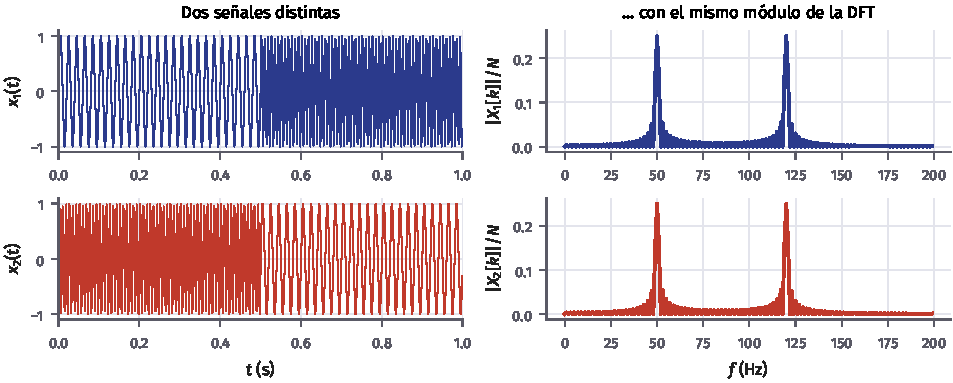
\includegraphics[width=\linewidth]{no_estacionaria}
  \caption{Dos señales distintas con el mismo módulo de la DFT.}\label{fig:no_estacionaria}
\end{figure}

La voz, la música, las vibraciones de una máquina que arranca o los ecos de un radar son \emph{no estacionarias}: su espectro cambia con el tiempo (en el Tema~6 se da una definición precisa de estacionariedad). Para estudiarlas se analiza la señal \emph{por tramos}: se multiplica por una ventana $w[n]$ de $L$ muestras colocada en cada instante y se calcula la DFT del tramo (\cref{fig:stft_tramos}). Como vimos en el Tema~3, multiplicar por una ventana es convolucionar el espectro de la señal con el de la ventana, así que conviene usar ventanas suaves (Hann, Hamming) y no la rectangular, cuyos lóbulos laterales son altos.

\begin{figure}[ht]
  \centering
  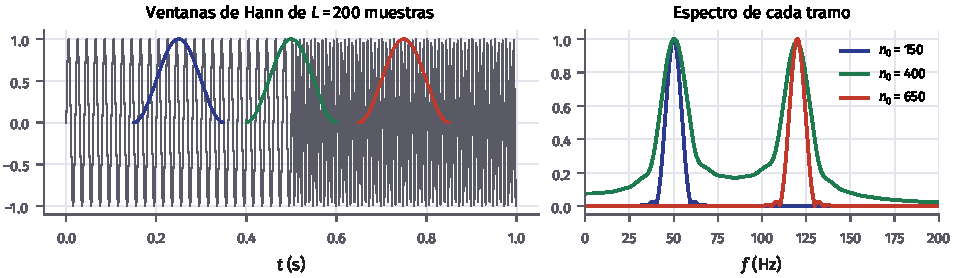
\includegraphics[width=\linewidth]{stft_tramos}
  \caption{Tres ventanas de Hann sobre la señal $x_1$ y el espectro de cada tramo. El tramo central contiene el cambio de frecuencia y muestra los dos tonos.}\label{fig:stft_tramos}
\end{figure}

\begin{nota}[Erratas de versiones anteriores]
  Las transparencias antiguas hablaban de «envenenamiento» de la señal donde quería decir \emph{enventanado}, y llamaban \texttt{espectrogram} a la función \texttt{spectrogram} de Matlab.
\end{nota}

\subsection{Definición}

\begin{definicion}{Transformada de Fourier de tiempo corto (STFT)}{stft}
  En tiempo continuo, con una ventana $w(t)$ desplazada a $\tau$,
  \[
    X(\tau,\omega)=\int_{-\infty}^{\infty}x(t)\,w(t-\tau)\,\e^{-j\omega t}\dd t .
  \]
  En tiempo discreto, con una ventana de $L$ muestras que avanza $R$ muestras de un tramo al siguiente,
  \[
    X(m,\Omega)=\sum_{n=-\infty}^{\infty}x[n]\,w[n-mR]\,\e^{-j\Omega n},
  \]
  y, muestreando la frecuencia con $N\ge L$ puntos, $X[m,k]=X(m,2\pi k/N)$, que se calcula con una DFT de $N$ puntos de cada tramo.
\end{definicion}

Para cada tramo $m$ hay un espectro, y para cada frecuencia $k$ una secuencia en el tiempo: la STFT es una función de dos variables. Con frecuencia de muestreo $f_s$, el tramo $m$ empieza en la muestra $mR$ y está centrado en $t_m=(mR+L/2)/f_s$, y el índice $k$ corresponde a $f_k=kf_s/N$. Algunos textos escriben la exponencial como $\e^{-j\Omega(n-mR)}$, es decir, miden el tiempo desde el principio de cada tramo; eso multiplica $X$ por $\e^{j\Omega mR}$, que cambia la fase pero no el módulo.

Si la ventana se anula fuera de $0\le n<L$, la suma tiene solo $L$ términos:
\[
  X[m,k]=\sum_{r=0}^{L-1}x[mR+r]\,w[r]\,\e^{-j2\pi k(mR+r)/N}.
\]

Para una señal de $N_x$ muestras, el número de tramos completos es
\[
  M=\left\lfloor\frac{N_x-L}{R}\right\rfloor+1 .
\]
Una señal real de 2\,s a $f_s=1$\,kHz con $L=128$, $R=32$ y $N=256$ da $M=\lfloor1872/32\rfloor+1=59$ tramos, y de cada uno basta guardar las $N/2+1=129$ frecuencias entre 0 y $f_s/2$.

\begin{encodigo}
  STFT calculada tramo a tramo para un chirp que barre de 50 a 400\,Hz en 2\,s. La frecuencia del máximo de cada tramo sigue la frecuencia instantánea $50+175t$\,Hz.
  \codigo{stft_manual}
\end{encodigo}

\subsection{Espectrograma}

El \emph{espectrograma} es el cuadrado del módulo de la STFT, $\abs{X[m,k]}^2$, representado sobre el plano tiempo-frecuencia con un mapa de colores, casi siempre en decibelios. En la \cref{fig:espectrograma} se distinguen tres componentes: el chirp aparece como una recta, el tono de 300\,Hz como un segmento horizontal entre 0,6 y 1,2\,s, y el clic de $t=1{,}6$\,s como una línea vertical, porque un impulso contiene todas las frecuencias. Las líneas verticales tenues en 0,6 y 1,2\,s son los transitorios del encendido y apagado brusco del tono.

\begin{figure}[ht]
  \centering
  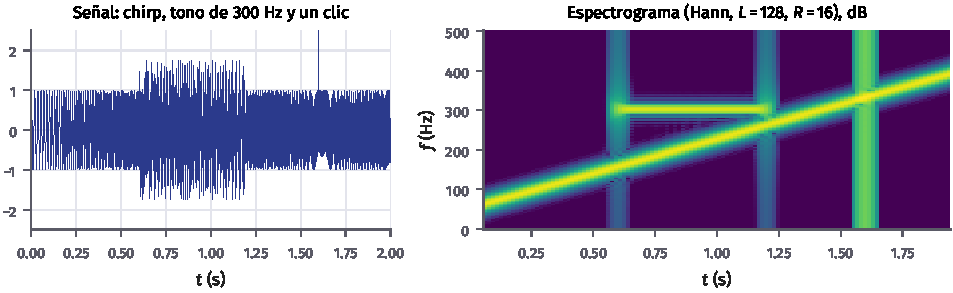
\includegraphics[width=\linewidth]{espectrograma_ejemplo}
  \caption{Señal de prueba y su espectrograma con una ventana de Hann de 128 muestras y salto de 16.}\label{fig:espectrograma}
\end{figure}

En Matlab el espectrograma lo calcula y dibuja \texttt{spectrogram(x, w, L-R, N, fs)}, cuyo tercer argumento es el solapamiento $L-R$; en Python, \texttt{scipy.signal.spectrogram} o la clase \texttt{ShortTimeFFT}. Octave no tiene \texttt{spectrogram}, sino \texttt{specgram}. Los ejemplos de estos apuntes calculan la STFT a mano para que se vea qué hacen.

\subsection{Resolución en tiempo y en frecuencia}

Los parámetros de la STFT son:
\begin{itemize}
  \item La \emph{longitud de la ventana} $L$, que fija la duración analizada, $\Delta t=L/f_s$, y la resolución en frecuencia. El lóbulo principal de una ventana de Hann mide $4f_s/L$ entre ceros, y dos tonos se distinguen si están separados al menos la mitad, $\approx2f_s/L$ (Tema~3).
  \item El \emph{tipo de ventana}, que reparte el compromiso entre la anchura del lóbulo principal y la altura de los secundarios.
  \item El \emph{salto} $R$ o, equivalentemente, el \emph{solapamiento} $L-R$. No cambia la resolución, sino lo densamente que se muestrea el eje de tiempos. Son habituales solapamientos del 50 al 75\,\%.
  \item El número de puntos de la DFT, $N\ge L$. Rellenar con ceros interpola el espectro, pero no separa mejor dos tonos.
\end{itemize}

La \cref{fig:resolucion} muestra el compromiso. Con $L=32$ (32\,ms) el clic y los bordes del tono quedan bien localizados, pero el lóbulo mide 125\,Hz y las frecuencias se emborronan. Con $L=512$ el tono de 300\,Hz es una raya fina, pero el chirp, que cambia 90\,Hz durante la ventana, se ensancha, y el clic se extiende medio segundo.

\begin{figure}[ht]
  \centering
  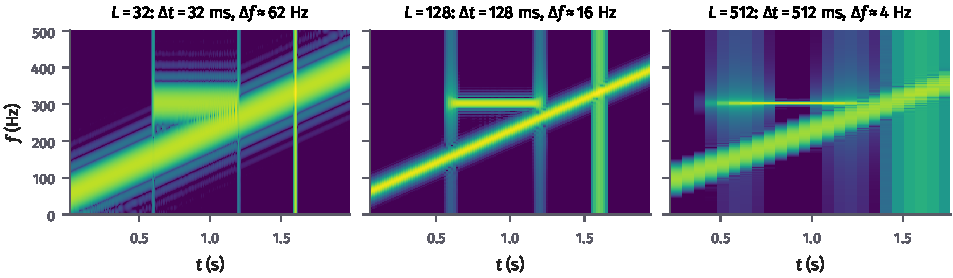
\includegraphics[width=\linewidth]{resolucion_tf}
  \caption{La misma señal con tres longitudes de ventana. $\Delta f$ es la separación mínima entre dos tonos para la ventana de Hann.}\label{fig:resolucion}
\end{figure}

Este compromiso es inevitable. Una señal de duración $\Delta t$ tiene un espectro de anchura del orden de $1/\Delta t$: es el \emph{principio de incertidumbre}. Si se miden las anchuras con las desviaciones típicas de $\abs{w(t)}^2$ y de $\abs{W(j\omega)}^2$ (normalizadas como densidades),
\[
  \sigma_t\,\sigma_\omega\ge\frac12,
\]
con igualdad solo para la ventana gaussiana. La STFT usa la misma ventana en todas las frecuencias, de modo que su resolución es la misma en todo el plano tiempo-frecuencia. La longitud se elige según la señal: en voz se usan 20–30\,ms, el tiempo durante el que el tracto vocal apenas cambia; en música, ventanas más largas para separar notas próximas.

\begin{ejemplo}{Una ventana imposible}{ventana-imposible}
  Con $f_s=1$\,kHz y ventana de Hann, separar dos tonos a 20\,Hz exige $2f_s/L\le20$, es decir, $L\ge100$ muestras (100\,ms). Separar dos clics a 10\,ms exige una ventana más corta que su separación, $L\lesssim10$. Ninguna longitud cumple ambas condiciones: hay que calcular dos espectrogramas o usar un análisis con resolución variable, como el de las wavelets (sección~\ref{sec:wavelets}).
\end{ejemplo}

\subsection{Síntesis por solapamiento y suma}

La STFT se puede invertir. La IDFT del tramo $m$ devuelve $x[n]\,w[n-mR]$; si se suman todos los tramos,
\[
  \sum_m x[n]\,w[n-mR]=x[n]\sum_mw[n-mR],
\]
que vale $C\,x[n]$ si las ventanas desplazadas suman una constante:
\[
  \sum_mw[n-mR]=C\qquad\text{para todo }n .
\]
Es la condición \emph{COLA} (\emph{constant overlap-add}), y el método se llama \emph{solapamiento y suma}. La cumplen la ventana de Hann periódica $w[n]=\frac12-\frac12\cos(2\pi n/L)$, $0\le n<L$, con $R=L/2$ (suma 1) o $R=L/4$ (suma 2), la de Hamming periódica con $R=L/2$ (suma 1,08) y la rectangular con $R=L$ (\cref{fig:cola}). Gracias a ella se puede modificar la señal en el plano tiempo-frecuencia (atenuar el ruido en los puntos donde domina, eliminar un tono durante un intervalo) y volver al tiempo. Es la base de muchos reductores de ruido y del \emph{vocoder} de fase, que cambia el tempo de una grabación sin cambiar su tono.

\begin{figure}[ht]
  \centering
  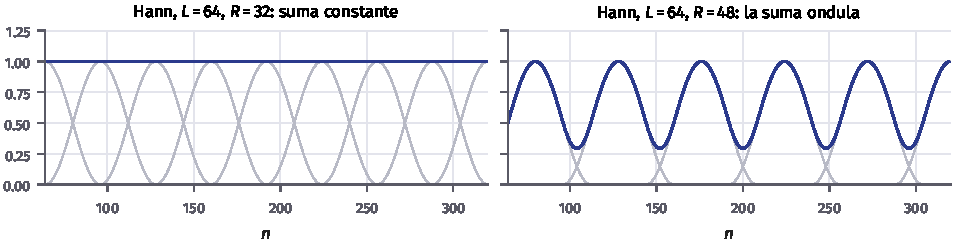
\includegraphics[width=\linewidth]{cola}
  \caption{Ventanas de Hann desplazadas (gris) y su suma (azul). Con $R=L/2$ la suma es constante; con $R=3L/4$, no.}\label{fig:cola}
\end{figure}

\begin{nota}[Ventana periódica y simétrica]
  La ventana de Hann \emph{simétrica} de longitud $L$, la de \texttt{hann(L)} en Matlab, tiene ceros en $n=0$ y $n=L-1$ y no cumple COLA exactamente. La \emph{periódica}, \texttt{hann(L,'periodic')}, es la simétrica de longitud $L+1$ sin la última muestra. Para analizar da igual; para resintetizar conviene la periódica.
\end{nota}

\subsection{Aplicaciones}

\paragraph{Marcación por tonos.} En la marcación DTMF cada tecla del teléfono suma una sinusoide de fila (697, 770, 852 o 941\,Hz) y una de columna (1209, 1336 o 1477\,Hz). El espectrograma de la \cref{fig:dtmf} muestra en qué instante se pulsó cada tecla y cuál: la «2» es $697+1336$\,Hz, el «0» $941+1336$ y el «5» $770+1336$. Para separar 697 y 770\,Hz, que distan 73\,Hz, una ventana de Hann necesita $L\ge2f_s/73\approx220$ muestras a 8\,kHz (27\,ms), menos que la duración mínima de un tono.

\begin{figure}[ht]
  \centering
  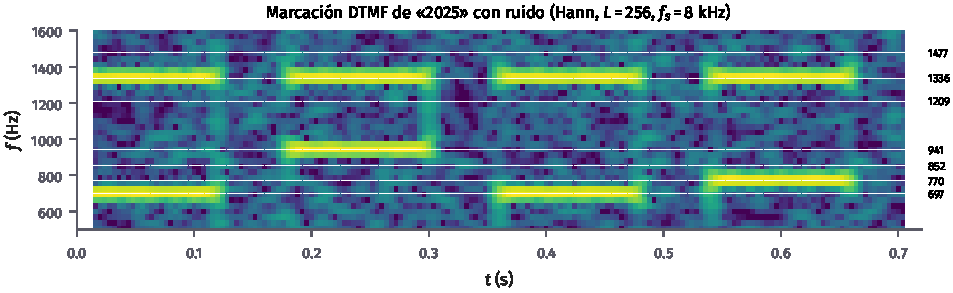
\includegraphics[width=\linewidth]{dtmf_espectrograma}
  \caption{Espectrograma de la marcación de «2025» con ruido.}\label{fig:dtmf}
\end{figure}

\begin{encodigo}
  Reconocimiento de una tecla a partir de 100\,ms de señal con ruido: se busca el máximo del espectro en la banda de las filas y en la de las columnas. Los receptores reales usan el algoritmo de Goertzel, que calcula solo las 7 componentes de la DFT que interesan.
  \codigo{dtmf}
\end{encodigo}

\paragraph{Otras aplicaciones.} En \emph{voz}, el espectrograma muestra los formantes (resonancias del tracto vocal) y el tono de la voz, y los reconocedores automáticos parten de una STFT. En \emph{música}, permite identificar notas e instrumentos. En \emph{mantenimiento predictivo}, el arranque de un motor es un chirp y un rodamiento dañado produce armónicos que crecen con el tiempo. En \emph{radar y sonar}, el desplazamiento Doppler a lo largo del tiempo revela la velocidad de un blanco.

\begin{flushright}\small\color{pdsgris}Ejercicios 1–5.\end{flushright}

% =====================================================================
\section{Wavelets}\label{sec:wavelets}

\subsection{De la STFT a las wavelets}

La STFT fija la ventana antes de analizar y la usa en todas las frecuencias. Pero muchas señales mezclan componentes lentas y largas (una tendencia, un tono grave) con detalles rápidos y breves (un clic, un salto, un borde). Lo natural sería analizar las bajas frecuencias con ventanas largas y las altas con ventanas cortas, de forma que cada análisis abarque aproximadamente el mismo número de periodos. Además, la sinusoide no siempre es la mejor forma con la que comparar: un latido del corazón o un escalón se parecen más a otras ondas.

La \cref{fig:teselas} resume la diferencia. Cada rectángulo representa la resolución de un coeficiente: la STFT reparte el plano en rectángulos iguales; las wavelets usan rectángulos estrechos y altos en alta frecuencia y anchos y bajos en baja frecuencia. El área es la misma en todos, como exige el principio de incertidumbre.

\begin{figure}[ht]
  \centering
  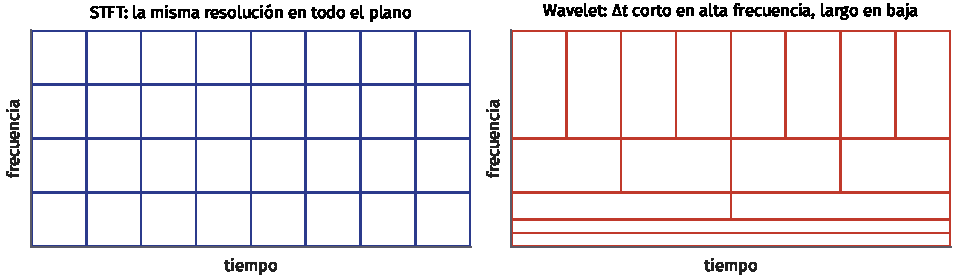
\includegraphics[width=\linewidth]{teselas}
  \caption{Reparto del plano tiempo-frecuencia de la STFT y de la transformada wavelet.}\label{fig:teselas}
\end{figure}

\subsection{Wavelets}

\begin{definicion}{Wavelet}{wavelet}
  Una \emph{wavelet madre} $\psi(t)$ es una función de energía finita, de duración limitada o que decae rápidamente, y de media nula. A partir de ella se forma la familia
  \[
    \psi_{a,b}(t)=\frac1{\sqrt a}\,\psi\!\left(\frac{t-b}a\right),\qquad a>0,\ b\in\R,
  \]
  donde $a$ es la \emph{escala} y $b$ el \emph{desplazamiento}. El factor $1/\sqrt a$ hace que todas tengan la misma energía.
\end{definicion}

La palabra significa «ondita»: oscila, como una sinusoide, pero solo durante un intervalo. Con $a<1$ la wavelet se comprime y oscila más deprisa; con $a>1$ se dilata (\cref{fig:escalado}). Si $\psi$ oscila con frecuencia $\omega_0$, $\psi_{a,b}$ oscila con $\omega_0/a$: la escala es inversamente proporcional a la frecuencia.

\begin{figure}[ht]
  \centering
  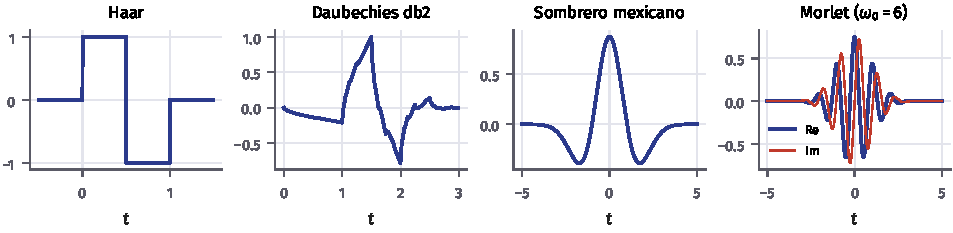
\includegraphics[width=\linewidth]{wavelets}
  \caption{Algunas wavelets madre. La de Morlet es compleja.}\label{fig:wavelets}
\end{figure}

\begin{figure}[ht]
  \centering
  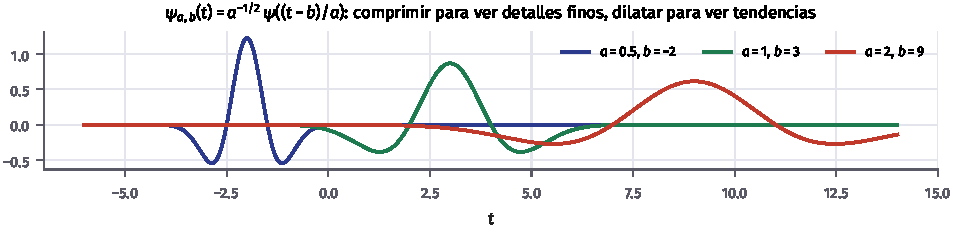
\includegraphics[width=\linewidth]{escalado_wavelet}
  \caption{Sombrero mexicano con tres escalas y desplazamientos.}\label{fig:escalado}
\end{figure}

Las wavelets más usadas (\cref{fig:wavelets}) son:
\begin{itemize}
  \item \emph{Haar}: $\psi(t)=1$ en $[0,\frac12)$, $-1$ en $[\frac12,1)$ y 0 en el resto. La más sencilla; discontinua.
  \item \emph{Daubechies} db$P$: soporte de longitud $2P-1$ y $P$ momentos nulos (véase más abajo); db1 es Haar. No tienen expresión cerrada: se definen por sus filtros.
  \item \emph{Sombrero mexicano}: la segunda derivada de una gaussiana cambiada de signo, $\psi(t)\propto(1-t^2)\e^{-t^2/2}$.
  \item \emph{Morlet}: una exponencial compleja con envolvente gaussiana, $\psi(t)=\pi^{-1/4}\e^{j\omega_0t}\e^{-t^2/2}$, normalmente con $\omega_0=6$. Es la más parecida a la STFT con ventana gaussiana.
\end{itemize}

\subsection{Transformada wavelet continua}

\begin{definicion}{Transformada wavelet continua}{cwt}
  \[
    W_x(a,b)=\int_{-\infty}^{\infty}x(t)\,\psi_{a,b}^*(t)\dd t=\frac1{\sqrt a}\int_{-\infty}^{\infty}x(t)\,\psi^*\!\left(\frac{t-b}a\right)\dd t .
  \]
\end{definicion}

$W_x(a,b)$ es la correlación de $x$ con la wavelet escalada, evaluada en $b$: mide cuánto se parece la señal, alrededor de $t=b$, a una onda de la forma de $\psi$ y anchura proporcional a $a$. La STFT correla con $w(t-\tau)\e^{j\omega t}$, que depende de tres parámetros (la posición, la frecuencia y la longitud de la ventana, fijada de antemano); la transformada wavelet, de dos.

El \emph{escalograma} es $\abs{W_x(a,b)}^2$ sobre el plano $(b,a)$. Se suele dibujar con la frecuencia equivalente en un eje logarítmico: para la Morlet, con $a$ en segundos, $f\approx\omega_0/(2\pi a)$. En la \cref{fig:escalograma} se compara con el espectrograma: el clic se estrecha al subir la frecuencia y el tono de 20\,Hz se resuelve en frecuencia mejor que el de 120\,Hz. Para la Morlet, la envolvente $\e^{-t^2/(2a^2)}$ tiene desviación típica $\sigma_t=a$ y su espectro, $\sigma_\omega=1/a$: el producto es constante y el área de cada «rectángulo» de la \cref{fig:teselas} también.

\begin{figure}[ht]
  \centering
  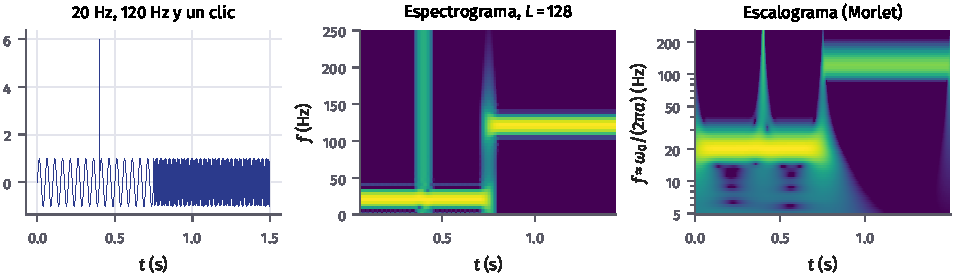
\includegraphics[width=\linewidth]{escalograma}
  \caption{Señal con un tono de 20\,Hz, uno de 120\,Hz y un clic: espectrograma y escalograma con la wavelet de Morlet.}\label{fig:escalograma}
\end{figure}

Para que la transformada se pueda invertir, $\psi$ debe cumplir la \emph{condición de admisibilidad}
\[
  C_\psi=\int_{-\infty}^{\infty}\frac{\abs{\Psi(j\omega)}^2}{\abs\omega}\dd\omega<\infty ,
\]
donde $\Psi(j\omega)$ es la CTFT de $\psi$. Si $\Psi$ es continua, la integral solo converge si $\Psi(j0)=0$, es decir, si $\int\psi(t)\dd t=0$: la wavelet tiene media nula y por tanto oscila. Entonces
\[
  x(t)=\frac1{C_\psi}\int_0^\infty\!\!\int_{-\infty}^{\infty}W_x(a,b)\,\psi_{a,b}(t)\,\frac{\dd b\,\dd a}{a^2}.
\]

\begin{definicion}{Momentos nulos}{momentos}
  Una wavelet tiene $P$ momentos nulos si
  \[
    \int_{-\infty}^{\infty}t^p\,\psi(t)\dd t=0,\qquad p=0,1,\dots,P-1 .
  \]
\end{definicion}

Si $\psi$ tiene $P$ momentos nulos, la transformada de cualquier polinomio de grado menor que $P$ es cero. Una señal suave se parece localmente a un polinomio, así que sus coeficientes son casi nulos en las escalas finas, y solo destacan las discontinuidades y los cambios bruscos. Haar tiene un momento nulo ($\int t\,\psi(t)\dd t=\frac18-\frac38=-\frac14\ne0$), el sombrero mexicano dos y db$P$, $P$.

\begin{nota}[Erratas de versiones anteriores]
  La admisibilidad aparecía con $\omega$ en el denominador, sin valor absoluto, y explicada como que $\abs{\Psi}^2$ «decae más rápidamente que $1/\omega$»; lo que exige en realidad es que $\Psi$ se anule en $\omega=0$. Los momentos nulos se definían con $p=0,\dots,N$ para «$N$ momentos», que son $N+1$ condiciones. Y se decía que la wavelet es «irregular y asimétrica», que no es una condición: el sombrero mexicano y la Morlet son simétricas.
\end{nota}

\subsection{Transformada wavelet discreta}

La CWT es muy redundante: una función de una variable se convierte en una de dos. Basta muestrear escalas y desplazamientos en una rejilla \emph{diádica}, $a=2^j$ y $b=k\,2^j$ con $j,k\in\Z$:
\[
  \psi_{j,k}(t)=2^{-j/2}\,\psi\!\left(2^{-j}t-k\right).
\]
Para wavelets bien elegidas (Haar, Daubechies y otras) estas funciones forman una \emph{base ortonormal}:
\[
  \int_{-\infty}^{\infty}\psi_{j,k}(t)\,\psi_{j',k'}(t)\dd t=\delta[j-j']\,\delta[k-k'] .
\]
Cualquier señal de energía finita se escribe entonces como
\[
  x(t)=\sum_{j}\sum_{k}d_j[k]\,\psi_{j,k}(t),\qquad d_j[k]=\int_{-\infty}^{\infty}x(t)\,\psi_{j,k}(t)\dd t ,
\]
y, por ser la base ortonormal, se cumple la igualdad de Parseval: $\int\abs{x(t)}^2\dd t=\sum_{j,k}\abs{d_j[k]}^2$.

\begin{nota}[Erratas de versiones anteriores]
  Las transparencias antiguas definían $\psi_{j,k}(t)=\psi(2^{-j}t-k)$, sin el factor $2^{-j/2}$, con lo que la base no es ortonormal, y escribían la ortonormalidad sin el $\dd t$ y con deltas de Dirac en lugar de deltas de Kronecker. En la descomposición por niveles llamaban a la señal unas veces $x(t)$ y otras $f(t)$.
\end{nota}

\paragraph{Análisis multirresolución.} Además de la wavelet se define una \emph{función de escala} $\varphi(t)$ (a veces llamada «wavelet padre»), de media 1, cuyas versiones $\varphi_{j,k}(t)=2^{-j/2}\varphi(2^{-j}t-k)$ recogen lo que queda de la señal por encima de una escala. Para Haar, $\varphi$ es el pulso rectangular de $[0,1)$. Se definen:
\begin{itemize}
  \item el \emph{detalle} del nivel $j$, $D_j(t)=\sum_kd_j[k]\,\psi_{j,k}(t)$, lo que la señal tiene a la escala $2^j$;
  \item la \emph{aproximación} del nivel $J$, $A_J(t)=\sum_ka_J[k]\,\varphi_{J,k}(t)$, con $a_J[k]=\int x(t)\varphi_{J,k}(t)\dd t$: la señal sin los detalles más finos que $2^J$.
\end{itemize}
Partiendo de una señal muestreada, que se identifica con la aproximación de nivel 0,
\[
  x=A_J+D_J+D_{J-1}+\dots+D_1,\qquad A_{j-1}=A_j+D_j .
\]
La \cref{fig:multiresolucion} muestra una descomposición de Haar en cuatro niveles: la aproximación $A_4$ conserva la forma general; los saltos aparecen en todos los detalles; la oscilación rápida del final, en $D_2$ y $D_3$.

\begin{figure}[ht]
  \centering
  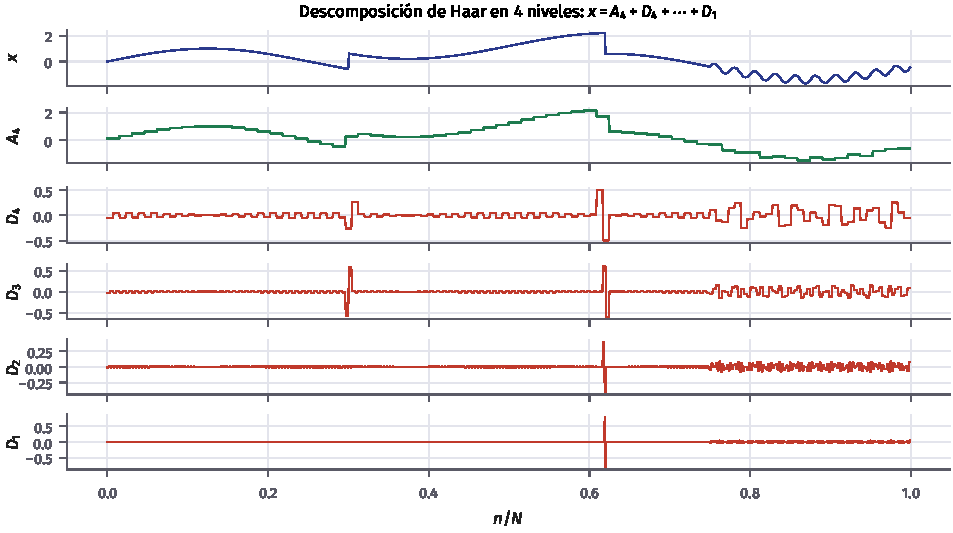
\includegraphics[width=\linewidth]{multiresolucion}
  \caption{Señal, aproximación y detalles de una descomposición de Haar en cuatro niveles. Cada componente tiene la longitud de la señal.}\label{fig:multiresolucion}
\end{figure}

\subsection{La DWT como banco de filtros}

$\varphi$ y $\psi$ cumplen las \emph{ecuaciones de dos escalas}
\[
  \varphi(t)=\sqrt2\sum_nh_0[n]\,\varphi(2t-n),\qquad\psi(t)=\sqrt2\sum_nh_1[n]\,\varphi(2t-n),
\]
donde $h_0$ es un filtro paso bajo y $h_1[n]=(-1)^nh_0[L-1-n]$ un paso alto de la misma longitud $L$. De ellas se deduce el \emph{algoritmo de Mallat}, que calcula los coeficientes de un nivel a partir de la aproximación del anterior sin calcular ninguna integral:
\[
  a_j[k]=\sum_nh_0[n-2k]\,a_{j-1}[n],\qquad d_j[k]=\sum_nh_1[n-2k]\,a_{j-1}[n].
\]
Es una convolución con $h_0[-n]$ y $h_1[-n]$ seguida de un \emph{diezmado por 2} (quedarse con una de cada dos muestras). La inversa intercala ceros (interpola por 2), filtra con $h_0$ y $h_1$ y suma.

\begin{propiedad}{DWT de Haar}{haar}
  Con $h_0=\frac1{\sqrt2}(1,1)$ y $h_1=\frac1{\sqrt2}(1,-1)$, un nivel de la DWT de una secuencia de longitud par es
  \[
    a_1[k]=\frac{x[2k]+x[2k+1]}{\sqrt2},\qquad d_1[k]=\frac{x[2k]-x[2k+1]}{\sqrt2},
  \]
  y la inversa,
  \[
    x[2k]=\frac{a_1[k]+d_1[k]}{\sqrt2},\qquad x[2k+1]=\frac{a_1[k]-d_1[k]}{\sqrt2}.
  \]
  La aproximación es la media de cada pareja (por $\sqrt2$) y el detalle, su semidiferencia.
\end{propiedad}

\begin{ejemplo}{Tres niveles de Haar}{haar3}
  Con $x=(4,6,10,12,8,6,5,5)$:
  \begin{itemize}
    \item Nivel 1: $a_1=\frac1{\sqrt2}(10,22,14,10)$, $d_1=\frac1{\sqrt2}(-2,-2,2,0)$.
    \item Nivel 2, sobre $a_1$: $a_2=\frac12(10+22,\,14+10)=(16,12)$, $d_2=\frac12(10-22,\,14-10)=(-6,2)$.
    \item Nivel 3: $a_3=\frac{28}{\sqrt2}=19{,}80$ y $d_3=\frac4{\sqrt2}=2{,}83$.
  \end{itemize}
  La energía se conserva: $\sum x^2=446$ y $392+8+(36+4)+\frac{4+4+4+0}2=446$. Casi toda está en $a_3$, la media.
\end{ejemplo}

Cada nivel parte la banda en dos (\cref{fig:banco_filtros}): $d_1$ recoge aproximadamente las frecuencias de $[\pi/2,\pi]$, $d_2$ las de $[\pi/4,\pi/2]$, y así hasta $a_J$, que recoge $[0,\pi/2^J]$. Los filtros de Haar separan mal las bandas; los de Daubechies más largos, mejor. En todos los casos $\abs{H_0}^2+\abs{H_1}^2=2$: la energía que uno quita la recoge el otro.

\begin{figure}[ht]
  \centering
  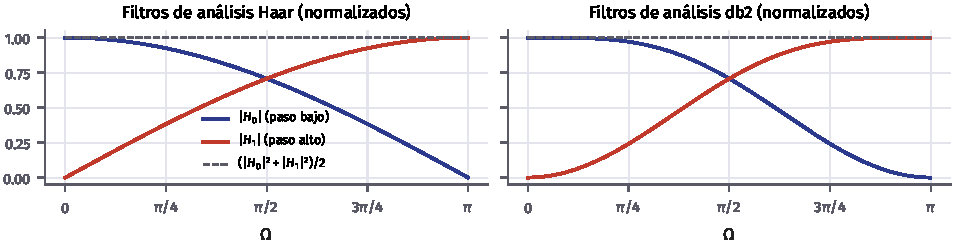
\includegraphics[width=\linewidth]{banco_filtros}
  \caption{Respuesta de los filtros de análisis de Haar y de db2.}\label{fig:banco_filtros}
\end{figure}

El número total de coeficientes es $\frac N2+\frac N4+\dots+\frac N{2^J}+\frac N{2^J}=N$: la DWT no añade redundancia, y el coste es $O(N)$, menor aún que el de la FFT. Los coeficientes del filtro db2 son
\[
  h_0=\frac1{4\sqrt2}\big(1+\sqrt3,\ 3+\sqrt3,\ 3-\sqrt3,\ 1-\sqrt3\big),
\]
y su paso alto $h_1$ cumple $\sum_nh_1[n]=0$ y $\sum_nn\,h_1[n]=0$: dos momentos nulos, de modo que los detalles de una rampa son nulos, salvo en los extremos. Con Haar, $x[n]=n$ da $d_1[k]=-1/\sqrt2$ en todos los $k$.

\begin{encodigo}
  DWT de Haar en cuatro niveles, comprobación de Parseval y de la reconstrucción. En Matlab, la Wavelet Toolbox ofrece \texttt{dwt}, \texttt{wavedec}, \texttt{waverec}, \texttt{wrcoef} y \texttt{cwt}; en Python, el paquete PyWavelets (\texttt{pywt.wavedec}, \texttt{pywt.cwt}).
  \codigo{haar_dwt}
\end{encodigo}

\subsection{Aplicaciones}

\paragraph{Eliminación de ruido.} La DWT concentra la energía de una señal con pocas discontinuidades en unos pocos coeficientes grandes, mientras que el ruido blanco, al ser la base ortonormal, reparte la suya por igual entre todos. Anulando los coeficientes de detalle pequeños y reconstruyendo se elimina gran parte del ruido. Hay dos reglas:
\[
  \text{umbral duro: }\ \hat d=\begin{cases}d,&\abs d>u\\0,&\abs d\le u\end{cases}\qquad
  \text{umbral suave: }\ \hat d=\sgn(d)\max(\abs d-u,0).
\]
Un umbral habitual es el universal de Donoho y Johnstone, $u=\hat\sigma\sqrt{2\ln N}$, con la desviación típica del ruido estimada a partir de los detalles más finos, que son casi todo ruido: $\hat\sigma=\operatorname{mediana}\abs{d_1[k]}/0{,}6745$. A diferencia de un paso bajo, que quita el ruido y también suaviza los saltos, el umbral conserva los saltos (\cref{fig:ruido}).

\begin{figure}[ht]
  \centering
  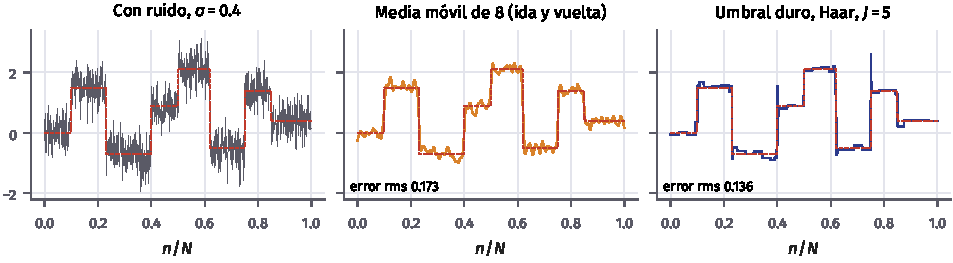
\includegraphics[width=\linewidth]{eliminacion_ruido}
  \caption{Señal escalonada con ruido, filtrada con una media móvil y con umbral sobre la DWT de Haar. En rojo, la señal sin ruido.}\label{fig:ruido}
\end{figure}

\begin{encodigo}
  Umbral duro sobre cinco niveles de Haar. El error cuadrático medio baja de 0,40 a 0,12.
  \codigo{eliminar_ruido}
\end{encodigo}

\paragraph{Compresión.} Si se guardan solo los coeficientes mayores, la señal se reconstruye con poco error (\cref{fig:compresion}). JPEG~2000 aplica una DWT bidimensional con wavelets biortogonales (la CDF 9/7) y codifica los coeficientes; a igual tamaño da menos artefactos que la DCT por bloques de JPEG.

\begin{figure}[ht]
  \centering
  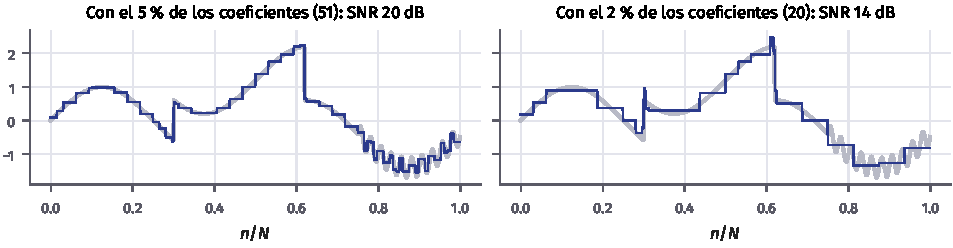
\includegraphics[width=\linewidth]{compresion}
  \caption{Reconstrucción a partir del 5 y del 2\,\% de los coeficientes de Haar.}\label{fig:compresion}
\end{figure}

\paragraph{Detección.} Los saltos y picos producen coeficientes grandes en todas las escalas, y las wavelets se usan para detectar los complejos QRS de un electrocardiograma o los fallos incipientes en una máquina. La elección de la wavelet depende de la forma de lo que se busca y del número de momentos nulos necesarios.

\begin{flushright}\small\color{pdsgris}Ejercicios 6–10.\end{flushright}

% =====================================================================
\section{Procesamiento de imágenes}\label{sec:imagenes}

\subsection{La imagen como señal bidimensional}

Una imagen es una señal que depende de dos variables espaciales. Una cámara la muestrea con una rejilla de sensores y cuantifica cada muestra: el resultado es una matriz $f[m,n]$ de $M\times N$ \emph{píxeles}, con $m=0,\dots,M-1$ la fila, contada de arriba abajo, y $n=0,\dots,N-1$ la columna (\cref{fig:pixeles}). En Matlab los índices empiezan en 1: el píxel $f[m,n]$ es \texttt{f(m+1, n+1)}.

\begin{figure}[ht]
  \centering
  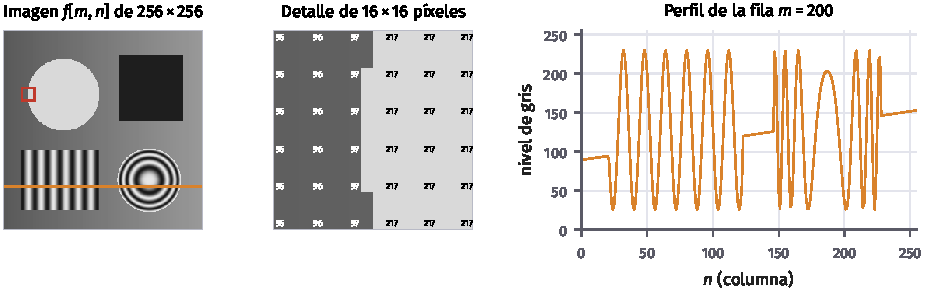
\includegraphics[width=\linewidth]{imagen_pixeles}
  \caption{La imagen de prueba de los ejemplos, un detalle de $16\times16$ píxeles con algunos de sus valores (de 0 a 255) y el perfil de una fila.}\label{fig:pixeles}
\end{figure}

\begin{itemize}
  \item \emph{Escala de grises}: un valor por píxel, entero de 8 bits (\texttt{uint8}, de 0, negro, a 255, blanco), de 16 bits, o real en $[0,1]$.
  \item \emph{Binaria}: 0 o 1.
  \item \emph{Color}: tres canales, normalmente rojo, verde y azul (RGB), es decir, una matriz de $M\times N\times3$. Hay otros espacios de color, como Lab (luminosidad y dos componentes de color) o YCbCr (el de JPEG).
\end{itemize}

El \emph{muestreo espacial} tiene las mismas reglas que el temporal (Tema~2): la frecuencia espacial se mide en ciclos por píxel, o por milímetro, y un detalle con periodo menor que dos píxeles produce \emph{aliasing}, el efecto moiré que aparece al fotografiar una tela de rayas finas. La \emph{cuantificación} con $b$ bits da $2^b$ niveles; con pocos niveles aparecen contornos falsos en los degradados.

Sin comprimir, una imagen ocupa $M\cdot N\cdot c\cdot b/8$ bytes, con $c$ canales: una imagen en color de $1920\times1080$ a 8 bits ocupa $6{,}2$\,MB. Por eso se guardan comprimidas: sin pérdidas (PNG, TIFF), eliminando redundancia, o con pérdidas (JPEG, JPEG~2000), descartando lo que menos se percibe. Matlab lee y escribe imágenes con \texttt{imread} e \texttt{imwrite} y las muestra con \texttt{imshow} o \texttt{image}; Python, con \texttt{matplotlib.pyplot.imread} e \texttt{imshow} o con el paquete Pillow.

\begin{encodigo}
  Los ejemplos usan una imagen sintética de $256\times256$ con un degradado, un círculo, un rectángulo, unas franjas verticales y un patrón de anillos, para no depender de ficheros externos.
  \codigo{imagen_prueba}
\end{encodigo}

\begin{nota}[Erratas de versiones anteriores]
  Las transparencias antiguas decían «Introducciónn», «repesentación» y «perdida» por «pérdida», y ponían «(ej: \emph{tiff})» como ejemplo de los formatos con pérdidas, además de los sin pérdidas.
\end{nota}

\subsection{Operaciones puntuales}

Una \emph{operación puntual} transforma cada píxel con una función de su propio valor, $s=T(r)$, sin mirar a los vecinos (\cref{fig:puntuales}). Con valores en $[0,1]$:
\begin{itemize}
  \item \emph{negativo}, $s=1-r$;
  \item \emph{corrección gamma}, $s=r^\gamma$: con $\gamma<1$ aclara los tonos oscuros, con $\gamma>1$ oscurece los claros;
  \item \emph{estiramiento lineal} del intervalo $[r_1,r_2]$ a $[0,1]$, recortando fuera de él (es lo que hace \texttt{imadjust} de Matlab);
  \item \emph{umbralización}, $s=1$ si $r>u$ y 0 si no, que da una imagen binaria.
\end{itemize}

\begin{figure}[ht]
  \centering
  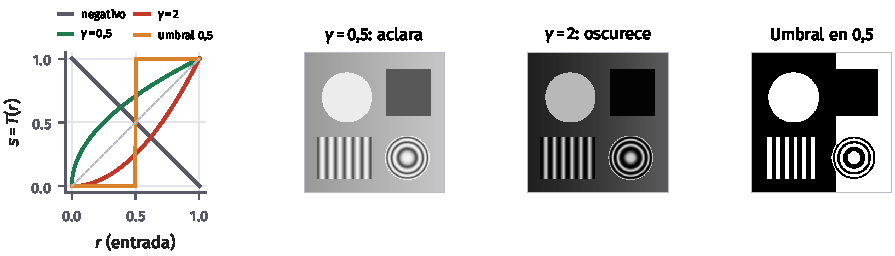
\includegraphics[width=\linewidth]{transformaciones_puntuales}
  \caption{Cuatro transformaciones puntuales y su efecto.}\label{fig:puntuales}
\end{figure}

\subsection{Histograma y ecualización}

\begin{definicion}{Histograma}{histograma}
  Si una imagen de $M\times N$ píxeles tiene $L$ niveles $r=0,\dots,L-1$, su \emph{histograma} $h[r]$ es el número de píxeles de nivel $r$. Normalizado, $p[r]=h[r]/(MN)$ es la proporción de píxeles de cada nivel, y
  \[
    F(r)=\sum_{i=0}^{r}p[i]
  \]
  es la proporción de píxeles con nivel menor o igual que $r$.
\end{definicion}

$p[r]$ y $F(r)$ son la función de probabilidad y la función de distribución del nivel de un píxel elegido al azar (Tema~6). Un histograma concentrado a la izquierda corresponde a una imagen oscura; a la derecha, a una clara; estrecho, a una con poco contraste. El histograma no dice dónde están los píxeles: dos imágenes muy distintas pueden tener el mismo. Si el objeto y el fondo tienen niveles distintos, el histograma tiene dos picos, y un umbral en el valle que los separa segmenta la imagen; el método de Otsu elige ese umbral automáticamente.

La \emph{ecualización} busca repartir los niveles por todo el rango con la transformación
\[
  s=T(r)=\operatorname{round}\big((L-1)\,F(r)\big),
\]
que es creciente, de modo que conserva el orden de los niveles. Si $r$ fuera una variable continua con función de distribución $F$, la variable $F(r)$ sería uniforme en $[0,1]$: es el mismo resultado que se usa en el Tema~6 para generar números aleatorios con una distribución dada. Con niveles discretos el histograma resultante no es plano (los píxeles de un mismo nivel van todos al mismo nivel nuevo), pero ocupa todo el rango (\cref{fig:ecualizacion}).

\begin{figure}[ht]
  \centering
  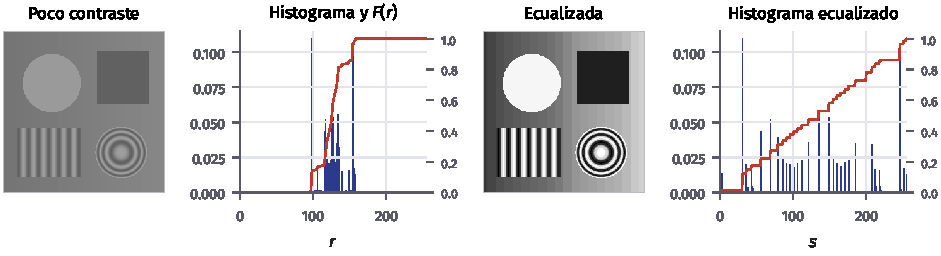
\includegraphics[width=\linewidth]{histograma_ecualizacion}
  \caption{Imagen con poco contraste, su histograma con $F(r)$ en rojo, la imagen ecualizada y su histograma.}\label{fig:ecualizacion}
\end{figure}

\begin{encodigo}
  Ecualización hecha a mano. Con la Image Processing Toolbox de Matlab, \texttt{imhist} dibuja el histograma e \texttt{histeq} ecualiza; \texttt{histeq} también puede llevar el histograma a una forma prefijada.
  \codigo{ecualizacion}
\end{encodigo}

\subsection{Convolución bidimensional}

\begin{definicion}{Convolución 2D}{conv2d}
  \[
    g[m,n]=(h\conv f)[m,n]=\sum_{i=-\infty}^{\infty}\sum_{j=-\infty}^{\infty}h[i,j]\,f[m-i,n-j].
  \]
\end{definicion}

Es la extensión directa de la convolución 1D, y como ella da la salida de un sistema lineal e invariante al desplazamiento cuya respuesta al impulso $\delta[m,n]$ es $h[m,n]$. En imágenes $h$ es casi siempre un \emph{núcleo} pequeño ($3\times3$, $5\times5$), es decir, un filtro FIR 2D, y cada píxel de salida es una combinación lineal de sus vecinos.

Si la imagen mide $M\times N$ y el núcleo $K\times K$, la convolución completa mide $(M+K-1)\times(N+K-1)$. Lo habitual es quedarse con la parte central del tamaño de la imagen (opción \texttt{'same'}) y, para los píxeles del borde, suponer algo sobre lo que hay fuera: ceros, el valor del borde repetido o la imagen reflejada. Rellenar con ceros oscurece el marco de la imagen.

El núcleo es \emph{separable} si $h[i,j]=u[i]\,v[j]$. Entonces basta filtrar cada fila con $v$ y después cada columna con $u$, con $2K$ productos por píxel en lugar de $K^2$: para $K=15$, 30 en vez de 225. El gaussiano y el de Sobel son separables.

\begin{nota}[Convolución y correlación]
  \texttt{conv2} de Matlab y \texttt{scipy.signal.convolve2d} calculan la convolución; \texttt{filter2} e \texttt{imfilter} de Matlab calculan la \emph{correlación}, $\sum_{i,j}h[i,j]f[m+i,n+j]$, que equivale a convolucionar con el núcleo girado 180°. Para núcleos simétricos dan lo mismo; para el de Sobel, el signo cambia.
\end{nota}

\begin{nota}[Erratas de versiones anteriores]
  La definición antigua de la convolución 1D escribía $(x*y)(m)$ en lugar de $(x*h)[m]$, y la de la 2D tenía un paréntesis de más y quedaba sin completar.
\end{nota}

\paragraph{Núcleos habituales.} (\Cref{fig:espaciales})
\begin{itemize}
  \item \emph{Media} de $K\times K$: $h=\frac1{K^2}$ en todo el núcleo. Paso bajo: reduce el ruido y emborrona los bordes. Su respuesta en frecuencia es un $\sinc$ con lóbulos secundarios.
  \item \emph{Gaussiano}: $h[i,j]\propto\e^{-(i^2+j^2)/(2\sigma^2)}$, normalizado para sumar 1. Paso bajo sin lóbulos ni artefactos; el más usado para suavizar.
  \item \emph{Sobel}:
  \[
    S_x=\begin{bmatrix}1&0&-1\\2&0&-2\\1&0&-1\end{bmatrix}=\begin{bmatrix}1\\2\\1\end{bmatrix}\begin{bmatrix}1&0&-1\end{bmatrix},
  \]
  una derivada horizontal ($f[m,n+1]-f[m,n-1]$, al convolucionar) combinada con un suavizado vertical; su traspuesta deriva en vertical. El módulo del gradiente $\sqrt{g_x^2+g_y^2}$ marca los bordes en cualquier dirección.
  \item \emph{Laplaciano}: $\begin{bsmallmatrix}0&1&0\\1&-4&1\\0&1&0\end{bsmallmatrix}$, aproximación de $\partial^2f/\partial m^2+\partial^2f/\partial n^2$. Paso alto: realza los detalles y también el ruido. Sumar a la imagen un múltiplo de $-\nabla^2f$ la hace más nítida.
\end{itemize}

\begin{figure}[ht]
  \centering
  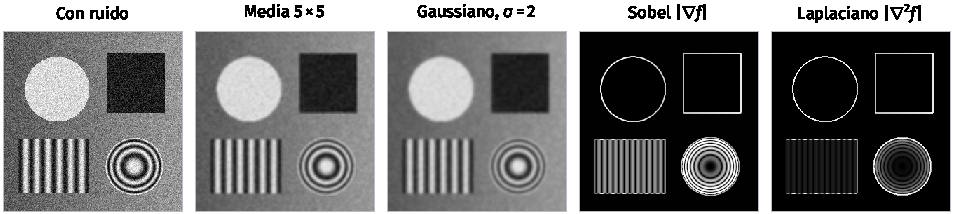
\includegraphics[width=\linewidth]{filtros_espaciales}
  \caption{Imagen con ruido suavizada con una media y con un gaussiano, y bordes de la imagen sin ruido detectados con Sobel y con el laplaciano.}\label{fig:espaciales}
\end{figure}

\begin{encodigo}
  Gradiente de Sobel. En el degradado la imagen crece $0{,}25/256$ por columna y $g_x$ vale ocho veces eso: el núcleo de Sobel da la derivada multiplicada por $2\times4$.
  \codigo{sobel}
\end{encodigo}

\subsection{DFT bidimensional}

\begin{definicion}{DFT 2D}{dft2}
  La DFT de una imagen $f[m,n]$ de $M\times N$ y su inversa son
  \[
    F[k,l]=\sum_{m=0}^{M-1}\sum_{n=0}^{N-1}f[m,n]\,\e^{-j2\pi\left(\frac{km}M+\frac{ln}N\right)},\qquad
    f[m,n]=\frac1{MN}\sum_{k=0}^{M-1}\sum_{l=0}^{N-1}F[k,l]\,\e^{j2\pi\left(\frac{km}M+\frac{ln}N\right)}.
  \]
\end{definicion}

La DFT 2D descompone la imagen en \emph{ondas planas} $\e^{j2\pi(km/M+ln/N)}$: franjas que tienen $k$ ciclos a lo largo de las filas y $l$ a lo largo de las columnas, orientadas perpendicularmente al vector $(k,l)$. $F[0,0]$ es la suma de todos los píxeles, y $F[0,0]/(MN)$ el nivel medio.

Como $\e^{-j2\pi(km/M+ln/N)}=\e^{-j2\pi km/M}\,\e^{-j2\pi ln/N}$, la DFT 2D es \emph{separable}:
\[
  F[k,l]=\sum_{m=0}^{M-1}\left[\sum_{n=0}^{N-1}f[m,n]\,\e^{-j2\pi ln/N}\right]\e^{-j2\pi km/M}:
\]
se calcula la DFT 1D de cada fila y después la de cada columna del resultado. Con la FFT cuesta $O(MN\log_2(MN))$. En Matlab y en Python, \texttt{fft2} e \texttt{ifft2}.

Para dibujarla se lleva el origen al centro con \texttt{fftshift} (las frecuencias $k\ge M/2$ son en realidad negativas) y se representa $\log(1+\abs{F})$, porque el valor en el origen es varios órdenes de magnitud mayor que el resto. La \cref{fig:dft2_patrones} muestra algunos casos: un coseno da dos puntos simétricos en la dirección perpendicular a sus franjas, tanto más alejados del centro cuanto más finas son, y un cuadrado da el producto de dos $\sinc$, con los lóbulos en cruz. En una imagen real (\cref{fig:dft2_imagen}) la energía se concentra en las bajas frecuencias, y los bordes rectos producen rayas perpendiculares a ellos.

\begin{figure}[ht]
  \centering
  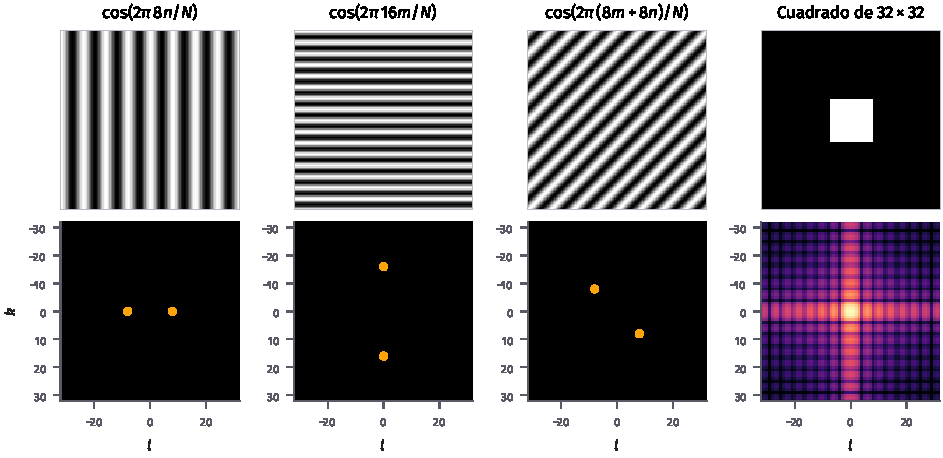
\includegraphics[width=\linewidth]{dft2_patrones}
  \caption{Cuatro imágenes de $128\times128$ y el módulo de su DFT centrada (zona central de $\pm32$).}\label{fig:dft2_patrones}
\end{figure}

\begin{figure}[ht]
  \centering
  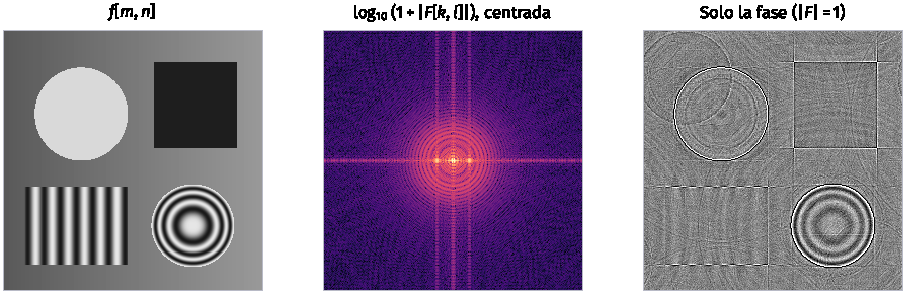
\includegraphics[width=\linewidth]{dft2_imagen}
  \caption{La imagen de prueba, el módulo de su DFT y la imagen que se obtiene conservando solo la fase.}\label{fig:dft2_imagen}
\end{figure}

\begin{propiedad}{Propiedades de la DFT 2D}{prop-dft2}
  \begin{itemize}
    \item \emph{Periodicidad}: $F[k+M,l]=F[k,l+N]=F[k,l]$, y lo mismo $f$ al invertir.
    \item \emph{Simetría}: si $f$ es real, $F[-k,-l]=F^*[k,l]$ (índices módulo $M$ y $N$), y $\abs F$ es simétrico respecto al origen.
    \item \emph{Desplazamiento circular}: $f[(m-m_0)_M,(n-n_0)_N]\parF\e^{-j2\pi\left(\frac{km_0}M+\frac{ln_0}N\right)}F[k,l]$. Mover la imagen no cambia $\abs F$.
    \item \emph{Rotación}: si se gira la imagen un ángulo $\theta$, su transformada (continua) gira el mismo ángulo.
    \item \emph{Convolución circular}: la convolución circular 2D de dos imágenes de $M\times N$ tiene por DFT el producto de sus DFT.
    \item \emph{Parseval}: $\sum_{m,n}\abs{f[m,n]}^2=\frac1{MN}\sum_{k,l}\abs{F[k,l]}^2$.
  \end{itemize}
\end{propiedad}

La periodicidad y la simetría son las que permiten centrar la DFT. La fase es tan importante como en 1D: en la \cref{fig:dft2_imagen}, la imagen reconstruida con $\abs F=1$ y la fase original conserva los bordes de los objetos, mientras que con el módulo y una fase cualquiera no se reconoce nada.

\begin{nota}[Erratas de versiones anteriores]
  La propiedad de desplazamiento aparecía como $\e^{-j2\pi(u\,m_0+v\,n_0)}F(u,v)$, sin dividir por $M$ y $N$. Se incluía una propiedad de escalado, $\DFT\{f(am,bn)\}=\frac1{ab}F(u/a,v/b)$, que es la de la transformada continua y no tiene sentido para la DFT. La separabilidad se escribía con factores $1/M$ y $1/N$ que no estaban en la definición, y la inversa como «$\IDFT(f(u,v))$» en lugar de $\IDFT\{F\}$. Además, la DFT 1D se presentaba como «FFT», que es el algoritmo que la calcula.
\end{nota}

\subsection{Filtrado en el dominio de la frecuencia}

Por el teorema de convolución, un filtro se puede aplicar multiplicando: $G[k,l]=H[k,l]\,F[k,l]$ y $g=\IDFT\{G\}$. Es la opción eficiente cuando el núcleo es grande. Dos precauciones: el producto de DFT corresponde a una convolución \emph{circular}, así que para obtener la lineal hay que rellenar con ceros hasta al menos $(M+K-1)\times(N+K-1)$; y para que $g$ sea real, $H$ debe tener la simetría $H[-k,-l]=H^*[k,l]$.

Con $D[k,l]=\sqrt{k^2+l^2}$ la distancia al origen (con las frecuencias negativas bien colocadas):
\begin{itemize}
  \item \emph{Paso bajo ideal}: $H=1$ si $D\le D_0$ y 0 si no. Su respuesta al impulso es la versión 2D de un $\sinc$, y produce \emph{anillos} alrededor de los bordes (el fenómeno de Gibbs del Tema~3).
  \item \emph{Paso bajo gaussiano}: $H=\e^{-D^2/(2D_0^2)}$. Su respuesta al impulso también es gaussiana, sin lóbulos: suaviza sin anillos. Corresponde a un gaussiano espacial de $\sigma=N/(2\pi D_0)$ píxeles (ejercicio~16).
  \item \emph{Paso alto}: $H_{\text{PA}}=1-H_{\text{PB}}$; deja los bordes.
\end{itemize}

\begin{figure}[ht]
  \centering
  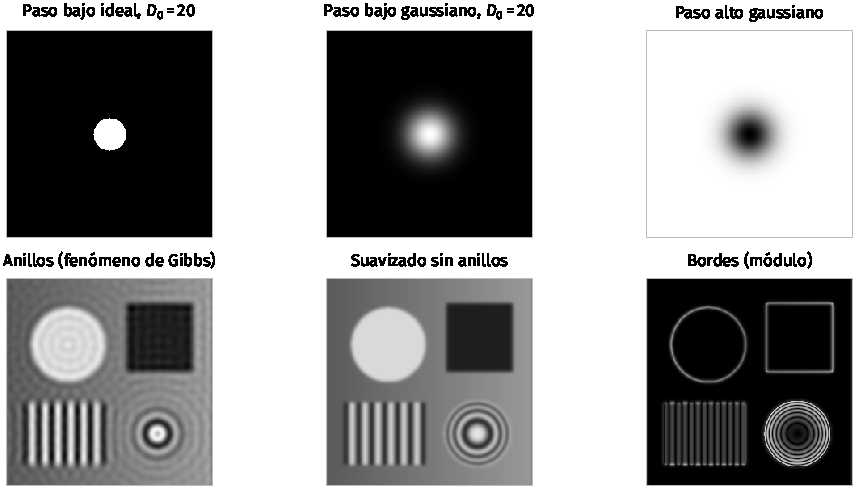
\includegraphics[width=\linewidth]{filtrado_frecuencia}
  \caption{Respuestas en frecuencia (centradas) y resultado de tres filtros aplicados con la DFT.}\label{fig:filtrado}
\end{figure}

\begin{encodigo}
  Paso bajo gaussiano con $D_0=20$ aplicado con la DFT. $H[0,0]=1$, así que el nivel medio no cambia; el filtro conserva el 96\,\% de la energía.
  \codigo{filtro_frecuencia_2d}
\end{encodigo}

\subsection{Otras aplicaciones}

\begin{itemize}
  \item \emph{Restauración}: si se conoce el desenfoque $H$ (por movimiento de la cámara, por ejemplo), se puede intentar deshacerlo dividiendo por $H$; donde $H\approx0$ esa división amplifica el ruido, y se usa el filtro de Wiener, que tiene en cuenta el espectro del ruido (Tema~6).
  \item \emph{Compresión}: JPEG divide la imagen en bloques de $8\times8$, aplica a cada uno la transformada discreta del coseno (DCT) y cuantifica con más fuerza las frecuencias altas; JPEG~2000 usa una DWT 2D.
  \item \emph{Segmentación y morfología}: umbralizar, detectar bordes, rellenar huecos y medir objetos.
  \item \emph{Visión por computador}: las redes neuronales convolucionales encadenan muchas convoluciones 2D cuyos núcleos se aprenden a partir de ejemplos.
\end{itemize}

\begin{flushright}\small\color{pdsgris}Ejercicios 11–16.\end{flushright}

% =====================================================================
\section*{Bibliografía}
\addcontentsline{toc}{section}{Bibliografía}

\begin{itemize}
  \item A.~V. Oppenheim y R.~W. Schafer, \emph{Tratamiento de señales en tiempo discreto}, 3.ª ed. Pearson, 2011. Capítulo 10 (análisis de Fourier de señales con la DFT, incluida la transformada de Fourier dependiente del tiempo).
  \item J.~G. Proakis y D.~G. Manolakis, \emph{Tratamiento digital de señales}, 4.ª ed. Pearson Prentice Hall, 2007. Capítulos de la DFT y de bancos de filtros.
  \item S.~Mallat, \emph{A Wavelet Tour of Signal Processing: The Sparse Way}, 3.ª ed. Academic Press, 2009. Referencia completa sobre wavelets, bancos de filtros y eliminación de ruido.
  \item R.~C. Gonzalez y R.~E. Woods, \emph{Digital Image Processing}, 4.ª ed. Pearson, 2018. Histograma, filtrado espacial, DFT 2D y filtrado en frecuencia, wavelets en imágenes.
  \item F.~T. Ulaby y A.~E. Yagle, \emph{Signals and Systems: Theory and Applications}, 2.ª ed. Michigan Publishing Services, 2024. Capítulos de procesamiento de imágenes y wavelets. Descarga libre en\\ \url{https://services.publishing.umich.edu/Books/S/Signals-and-Systems}.
\end{itemize}

\end{document}
